\chapter{Mathematical background}

The theory of elliptic curves is at the foundation of isogeny-based Cryptography, but in a very different style from classical Elliptic Curve Cryptography: the latter uses the group of points of a single curve, while the first uses graphs of elliptic curves.

Our introduction on these topics will follow \cite{Silverman} and \cite{DeFeo_intro}.

\section{Elliptic curves}

We start by giving the most general definition of an elliptic curve over a field $K$.

\begin{definition}
    An \emph{elliptic curve} $E$ \emph{over} $K$ is a smooth projective curve of genus $1$, with a given $K$-rational point.
\end{definition}

Since we will work over finite fields of large characteristic, we will assume in all our theorems that $\car K\neq 2,3$. This allows us to simplify the representation of an elliptic curve.

\begin{proposition}[Weierstrass model]
    Let $E$ be an elliptic curve over $K$, with $\car K\neq 2,3$. Then there exist $a,b\in K$ with $4a^3+27b^2\neq0$ such that $E$ is isomorphic to the curve $$ZY^2=X^3+aXZ^2+bZ^3.$$
    
    The point $O=(0:1:0)$ is called the \emph{point at infinity} of $E$, and it's the only point on $Z=0$.
\end{proposition}

Usually we then identify the curve with its affine patch at $Z\neq0$, i.e. with the equation $$y^2=x^3+ax+b,$$
plus the point at infinity $O$.

Any elliptic curve can (almost) be identified by a single number, the \emph{$j$-invariant}:
\begin{theorem}
    Let $E:y^2=x^3+ax+b$ be an elliptic curve over $K$, and let its $j$-invariant be $$j(E)=1728\frac{4a^3}{4a^3+27b^2}.$$
    
    Then any other elliptic curve $E'$ is isomoprhic to $E$, over $\bar K$, if and only if $j(E)=j(E')$.
\end{theorem}

We will make precise sense of what ``almost" and ``isomorphic" means in the next sections when we will introduce isogenies and twists.

Elliptic curves are also well known for naturally having a structure of abelian group, with the point at infinity $O$ as the neutral element.

\begin{theorem}
    Let $E$ be an elliptic curve over $K$, given by a Weierstrass equation $y^2=x^3+ax+b$. Then there exists an abelian group law $\oplus$ on the set of $L$-rational points $E(L)$ for any field extension $K\subset L$.
    
    Given affine points $P_1=(x_1,y_1)$ and $P_2=(x_2,y_2)$ the addition law is defined by:
    \begin{itemize}
        \item If $x_1=x_2$ and $y_1=-y_2$, then $P_1\oplus P_2=O$.
        \item Otherwise $P_1\oplus P_2=(x_3,y_3)$ with \begin{align*}
            x_3 &=  \lambda^2-x_1-x_2\\
            y_3 &= -\lambda x_3-y_1+\lambda x_1
        \end{align*}
        where $\lambda=\frac{3x_1^2+a}{2y_1}$ if $P_1=P_2$, and $\lambda=\frac{y_2-y_1}{x_2-x_1}$ otherwise.
    \end{itemize}
\end{theorem}\todo{maybe usual picture?}

The structure of this group has been much studied, and there are still open questions; luckily we will work in finite fields, where most of it is understood.

\begin{theorem}
    Let $E$ be an elliptic curve over an algebraically closed field $K$ of characteristic $p$, and let $m$ be an integer. Then the $m$-torsion group of $E(K)$, denoted by $E[m]$, is given by:
    \begin{itemize}
        \item $E[m]\cong \Zn{m}\times\Zn{m}$, if $p$ does not divide $m$.
        \item If $p>0$, then either $E[p^r]\cong\Zn{p^r}$ for all $r\ge0$ or $E[p^r]=\{O\}$.
    \end{itemize}
\end{theorem}

The curves where the last case happens are called \emph{supersingular}, and they are one of the main topics of this thesis.

\begin{theorem}
    Let $E$ be an elliptic curve over a field $K$. Then
    \begin{itemize}
        \item If $K$ is a number field, then $E(K)$ is a finitely generated abelian group.
        \item If $K=\F_q$, then $E(\F_q)\cong\Zn{n}\times\Zn{m}$, with $n\mid\gcd(m, q-1)$.
    \end{itemize}
\end{theorem}

The determination of the rank of $E(K)$ in the number field case is the focal point of the Birch and Swinnerton-Dyer conjecture, which is one of the Millennium Problems. It is also unknown if such rank is bounded or unbounded for elliptic curves over $\Q$.

\section{Isogenies}

Since elliptic curves are algebraic varieties, we briefly recall some notions of maps between varieties.

\begin{definition}
    Let $V_1,V_2$ be projective varieties over an algebraically closed field $\bar K$, and $\bar K(V_1), \bar K(V_2)$ their function fields.
    
    A \emph{rational map} $\phi:V_1\to V_2$ is $\phi=[f_1,\dots,f_n]$, where $f_i\in\bar K(V_1)$ such that for any point $P$ at which all $f_i$ are defined we have $\phi(P)=[f_1(P),\dots,f_n(P)]\in V_2$.
    
    A \emph{morphism} is a rational map that is regular at any point, i.e. for any $P\in V_1$ there exists a function $g\in\bar K(V_1)$ such that all $gf_i$ are defined at $P$, and at least one $gf_i(P)\neq0$.
\end{definition}
\todo{examples}

A very important property of morphisms is the following:
\begin{proposition}
    Let $\phi: V_1\to V_2$ be a morphism of projective varieties defined over $K$, with $\phi=[f_1,\dots,f_n]$. Then the map $\phi^\ast:K(V_2)\to K(V_1)$ given by $\phi^\ast(g)(x)=g(f_1(x),\dots,f_n(x))$ is a homomorphism of $K$-algebras.
\end{proposition}

We now turn our attention to curves, which are varieties of dimension $1$, for example all polynomials $f(x,y)=0$ in two variables.

Since we will work over finite fields, it's important to clearly state the definition of separable and inseparable morphisms.

\begin{definition}
    Let $\phi:C_1\to C_2$ be a nonconstant morphism of curves defined over $K$. Then we define its \emph{degree} to be $$\deg\phi = [K(C_1):\phi^\ast K(C_2)].$$
    Moreover we say that $\phi$ is \emph{separable}, \emph{inseparable} or \emph{purely inseparable} exactly when the extension of function fields is. Finally, we define $\deg_s\phi$ and $\deg_i\phi$ as the separable and inseparable degree of the field extension.
\end{definition}

A geometric interpretation of (separable) degree is the following, and in some sense it shows why it is the ``right" definition:

\begin{proposition}
    Let $\phi: C_1\to C_2$ be a morphism between smooth curves defined over $\bar K$. Then $\#\phi^{-1}(Q)=\deg_s\phi$ for all but finitely many $Q\in C_2$.
\end{proposition}

Turning back to elliptic curves, we are ready to define \emph{isogenies}.
\begin{definition}
    Let $E_1$ and $E_2$ be elliptic curves, with points at infinity $O_1,O_2$. An \emph{isogeny} is a morphism of curves $\phi:E_1\to E_2$ such that $\phi(O_1)=O_2$.
    
    We denote the set of isogenies from $E_1$ to $E_2$ by $\Hom(E_1, E_2)$.
\end{definition}

\begin{example}
    We set $E_1:y^2=x^3+x$ and $E_2:y^2=x^3-4x$. Then the map $\phi:E_1\to E_2$ defined by $$\phi(x,y)=\left(\frac{x^2+1}{x}, y\frac{x^2-1}{x^2}\right), \;\phi(0,0)=O$$ is a separable isogeny of curves over $\Q$. Its kernel has size $2$ and is generated by $(0,0)$.
    
    It is indeed a morphism, since in projective coordinates it can be written as
    \begin{align*}
    \phi(X:Y:Z) &= (X(X^2+Z^2):Y(X^2-Z^2):X^2Z)\\
    &= (Y(X^2+Z^2):XY^2-X^2Z-Z^3:XYZ)
    \end{align*}
    and is defined even at $(0:0:1)$.
\end{example}

Notice that $\Hom(E_1, E_2)$ is a group, with neutral element the constant isogeny that sends everything to $O_2$.

Moreover, the choice of the $\Hom$ notation is not random: it turns out that isogenies are the right morphisms for the category of elliptic curves, since we have the following:
\begin{proposition}
    Let $\phi:E_1 \to E_2$ be a nonconstant isogeny. Then $\phi$ induces a surjective group homomorphism $E_1(\bar K)\to E_2(\bar K)$ with finite kernel.
    
    In particular, $\#\ker \phi = \deg_s\phi = \#\phi^{-1}(Q)$ for \emph{any} $Q\in E_2(\bar K)$.
\end{proposition}

It turns out that the kernel of a separable isogeny completely determines it, and we have simple formulas to evaluate the resulting isogeny, due to Vélu.
\begin{proposition}
    Let $E$ be an elliptic curve over an algebraically closed field $\bar K$, and $G$ a subgroup of $E(\bar K)$. Then there is a curve $E'$ and a separable isogeny $\phi:E\to E'$ with $\ker\phi=G$; the curve and the isogeny are unique up to isomorphisms $E'\cong E''$.
    
    If $E$ is defined by the equation $y^2=x^3+ax+b$, then $E'$ has equation $y^2=x^3+a'x+b'$, where
    \begin{align*}
    a' &= a-5\sum_{Q\in G\setminus\{O\}}(3x(Q)^2+a)\\
    b' &= b-7\sum_{Q\in G\setminus\{O\}}(5x(Q)^2+3ax(Q)+2b)
    \end{align*}
    and for any $P\in E(\bar K)$ we have
    $$\phi(P) = \left(x(P) + \sum_{Q\in G\setminus\{O\}} x(P+Q)-x(Q), y(P)+ \sum_{Q\in G\setminus\{O\}} y(P+Q)-y(Q)\right)$$
\end{proposition}

Notice that, given these formulas, both the resulting curve and a point evaluation can be computed in $O(\# G)$ time.\todo{maybe explicit example}

One of the most important example of isogenies is multiplication-by-$m$:
\begin{example}
    For any $m\in\Z$ we have a natural isogeny $[m]:E\to E$, which we can define by induction with $[0](P)=O$, $[m+1]P=[m]P\oplus P$ and $[-m](P)=[m](-P)$. Since addition and negation are morphisms of curves, this actually defines an isogeny.
    
    We can show that $[m]$ is nonconstant, and its kernel is $E[m]$, for which we have stated its structure; most importantly, we observe that $\deg[m]=m^2$, which is a fundamental result in the theory of dual isogenies.
\end{example}

Indeed, we now define dual isogenies and state their properties

\begin{theorem}
    Let $\phi:E_1\to E_2$ an isogeny of degree $d$. Then there exists a unique isogeny $\hat\phi:E_2\to E_1$ such that $\hat\phi \phi=[d]$.
    
    $\hat\phi$ is called the \emph{dual isogeny} of $\phi$ and has the following properties:
    \begin{enumerate}
        \item Also $\phi\hat\phi=[d]$, the multiplication-by-$d$ on $E_2$.
        \item $\hat\phi$ has also degree $d$.
        \item $\hat\phi$ is defined over $K$ if and only if $\phi$ is.
        \item $\widehat{\psi\circ\phi}=\hat\phi\circ\hat\psi$ for any isogeny $\psi:E_2\to E_3$.
        \item $\widehat{\psi + \phi}=\hat\psi + \hat\phi$ for any isogeny $\psi:E_1\to E_2$.
        \item $\hat{\hat\phi}=\phi$.
    \end{enumerate}
\end{theorem}

Notice that this implies $\widehat{[m]}=[m]$, and thus that $\deg[m]=m^2$ as we already said.

(Splitting lemma?)

Standard form/division polynomials?\todo{write this}

\section{Endomorphisms and automorphisms}

In the previous section we observed that $\Hom(E_1, E_2)$ is a group because isogenies can be added. Notice that if $E_1=E_2=E$ we can also compose isogenies; thus we get the ring $\End(E)$. We clearly have $\Z\subset\End(E)$, identifying $\Z$ with the multiplication-by-$m$ isogenies; however the endomorphism ring can be bigger, and it will play a central role in isogeny-based cryptography.

First we focus on \emph{invertible} isogenies, i.e. isomorphisms, since they are very easy to describe. In particular
\begin{proposition}
    Let $E:y^2=x^3+ax+b$ and $E':{y'}^2={x'}^3+a'x'+b'$ be two elliptic curves in Weierstrass form; the only isomorphisms between them are of the form $(x',y')=(u^2x, u^3y)$, which implies $a'=au^4$ and $b'=bu^6$.
\end{proposition}

This means that the group $\Aut(E)$ of invertible endomorphisms is easily computable and helps to understand the failure of the $j$ invariant to classify the isomorphism classes.

\begin{theorem}
    Let $E/\bar K$ be an elliptic curve and $\car K\neq 2,3$. Then $\Aut(E)\cong\mu_n$, where $\mu_n$ is the group of the $n$ roots of unity in $\bar K$ and 
    $$n=\begin{cases}2\text{ if } j\neq0,1728\\ 4 \text{ if } j=1728\\ 6 \text{ if } j=0\end{cases}$$
    The automorphism corresponding to $\zeta\in\mu_n$ is $(x,y)\mapsto(\zeta^2x,\zeta^3y)$, if $E$ is given in Weierstrass form.
\end{theorem}

Observe that except the two particular curves with $j=0$ or $1728$, the only non-trivial automorphism is $[-1]$.

Moreover this computation of the automorphism group can be used to obtain a classification of \emph{twists}.

\begin{definition}
    Let $E$ be an elliptic curve over $K$. A \emph{twist} of $E$ is an elliptic curve $E'/K$ with $j(E)=j(E')$, but which is not necessarily isomorphic to $E$ over $K$.
\end{definition}\todo{example?}

The classification of all twists of a curve in Weierstrass form is then the following:
\begin{proposition}
    Let $E:y^2+ax+b$ be an elliptic curve over $K$. Then the set of twists of $E$, modulo $K$-isomorphism, is canonically isomorphic to $K^\ast/{K^\ast}^n$, with $n$ as before.
    
    In particular, given $d\in K^\ast/{K^\ast}^n$, the twist $E_d$ corresponding to $d$ is:
    \begin{itemize}
        \item $E_d: y^2=x^3+d^2ax+d^3b$ for $j(E)\neq0,1728$.
        \item $E_d: y^2=x^3+dax$ for $j(E)=1728$.
        \item $E_d: y^2=x^3+db$ for $j(E)=0$.
    \end{itemize}
\end{proposition}

We now go back to endomorphisms. One fundamental result is one that bounds the size of $\Hom(E_1,E_2)$:
\begin{proposition}
    Let $E_1,E_2$ be elliptic curves. Then the $\Z$-module $\Hom(E_1,E_2)$ is torsion-free and has rank at most $4$.
\end{proposition}

In particular, we have very few possibilities for the endomorphism ring:
\begin{theorem}
    Let $E$ be an elliptic curve defined over $K$. Then its full endomorphism ring is one of the following:
    \begin{itemize}
        \item $\End(E)\cong\Z$.
        \item $\End(E)$ is an order in an imaginary quadratic number field.
        \item $\End(E)$ is a maximal order in a quaternion algebra.
    \end{itemize}
\end{theorem}

When $\car K=0$, usually we have only the scalars, but sometimes $\End(E)$ has rank 2, in which case we say it has \emph{complex multiplication}.

Over finite fields, every curve has at least the Frobenius endomorphism; in some very special cases it happens that $\End(E)$ has rank 4. These curves are again the \emph{supersingular} curves we have met above.

Notice that in this case $\End(E)$ is non commutative; the difficulty of explicitly finding these extra endomorphisms is one of the hardness assumptions on which isogeny crypto is founded.


\section{Elliptic curves over finite fields}

In this section we shift the focus towards elliptic curves defined over some $\F_q$, which is the usual setting used in cryptography.

Probably the most important object in studying elliptic curves over finite fields is the \emph{Frobenius endomorphism}, and in general Frobenius isogenies.

\begin{definition}
    Let $E/K$ be an elliptic curve over a field of characteristic $p$, given by a Weierstrass equation $y^2=x^3+ax+b$. For any $q=p^r$ define $E^{(q)}$ to be the elliptic curve $y^2=x^3+a^qx+b^q$ and $\pi_q:E\to E^{(q)}$ to be the isogeny $$\pi_q(X:Y:Z)=(X^q:Y^q:Z^q).$$
    
    In particular, if $E$ is defined over $\F_q$, then $E^{(q)}=E$ and $\pi_q$ is an endomorphism of $E$, called the Frobenius endomorphism and usually denoted simply by $\pi$.
\end{definition}

A generic Frobenius isogeny can be proved to have the following properties:
\begin{proposition}
    Let $\pi_q:E\to E^{(q)}$ be the Frobenius isogeny. Then $\pi_q$ is purely inseparable, has degree $q$ and $\ker\pi_q = \{O\}$.
\end{proposition}

Much like field theory, where any extension can be split into a separable part and a purely inseparable part, the Frobenius isogeny helps us decompose arbitrary isogenies.
\begin{proposition}
    Let $\phi: E\to E'$ be an isogeny of elliptic curves defined over a field of characteristic $p$. Then $\phi$ can be written as the composition of a Frobenius isogeny $\pi_q:E\to E^{(q)}$ and a separable isogeny $\phi_s:E^{(q)}\to E'$.
    
    \[\begin{tikzcd}
        E\rar["\pi_q"] \ar[rr, bend right, "\phi"] & E^{(q)} \rar["\phi_s"] & E'
    \end{tikzcd}\]
\end{proposition}

Turning back to the special Frobenius endomorphism, one of the first clues of its fundamental influence on the curve is the following
\begin{proposition}
    Let $E/\F_q$ be an elliptic curve and $\pi$ its Frobenius endomorphism. Then $\ker(\pi-1) = E(\F_q)$, i.e. the points fixed by the Frobenius are precisely the $\F_q$-rational points.
\end{proposition}

However the most important feature of the Frobenius endomorphism is its \emph{trace}, which is tightly correlated with the point-counting function of the elliptic curve.

\begin{theorem}
    Let $E/\F_q$ be an elliptic curve and $\pi$ its Frobenius endomorphism. Then there exists $t\in\Z$ such that $$\pi^2-t\pi+q=0.$$
    
    Moreover, if $\alpha,\beta$ are the roots of $X^2-tX+q=0$ we have that $|\alpha|=|\beta|=\sqrt q$ and $$\# E(\F_{q^n}) = q^n+1-\alpha^n-\beta^n$$
    
    In particular, $\# E(\F_q) = q+1-t$ with $|t|\le2\sqrt q$.
\end{theorem}

This powerful theorem is actually the simplest case of the famous Weil's conjectures, which are a major cornerstone of arithmetic geometry.

It turns out that the number of points is also invariant by isogenies, which is a theorem due to Tate:
\begin{theorem}
    Let $E_1,E_2$ be elliptic curves defined over $\F_q$. Then there exists an isogeny $\phi: E_1\to E_2$ defined over $\F_q$ if and only if $\# E_1(\F_q)=\# E_2(\F_q)$.
\end{theorem}

Notice that counting the number of points is an easy problem, due to the Schoof-Elkies-Atkin algorithm, which has a heuristic running time of $O(\log^4 q)$.

The problem of deciding whether $E_1$ and $E_2$ are isogenous \emph{with a degree $\ell$ isogeny} is also somewhat feasible, with very similar techiniques to the SEA algorithm, namely the use of \emph{modular polynomials}.

\begin{theorem}
    For any prime $\ell$ there exists a symmetric polynomial $\Phi_\ell\in\Z[x,y]$, of degree $\ell+1$ in each wariable, such that two elliptic curves $E_1,E_2$ defined over an algebraically closed field are $\ell$-isogenous if and only if $\Phi_\ell(j(E_1),j(E_2))=0$.
\end{theorem}

These polynomials are independent from the base field (in particular they work both in positive and zero characteristic) and thus can be precomputed. They have $O(\ell^2)$ coefficients, and each of them grows very fast in size, so this decision problem is only solvable for ``small" values of $\ell$.

Moreover, the modular polynomials can be used to compute all $\ell$-isogenous curves from a given $E$ by simply finding the roots of the univariate polynomial $\Phi_\ell(j(E),y)=0$. In particular, finding roots over a field $K$ will give $K$-rational isogenies.

\begin{example}
    The modular polynomials for degrees $2$ and $3$ are as follows:
    \begin{align*}
    \Phi_2(X,Y) &= (X+Y)^3-X^2Y^2+1485XY(X+Y)-162000(X+Y)^2 \\
    & + 41097375 XY + 8748000000(X+Y) - 157464000000000
    \end{align*}
    \begin{align*}
    \Phi_3(X,Y) &= (X+Y)^4 - X^3Y^3 + 2232X^2Y^2(X+Y) + 36864000(X+Y)^3\\
    & - 1069960XY(X+Y)^2 + 2590058000X^2Y^2\\
    & + 8900112384000XY(X+Y) + 452984832000000(X+Y)^2\\
    & - 771751936000000000XY + 1855425871872000000000(X+Y)
    \end{align*}
\end{example}

Finally, we make a remark on twists over finite fields: since the multiplicative group $\F_q^\ast$ is cyclic, there is exactly one quadratic twist of an elliptic curve.
\begin{proposition}
    Let $E/\F_q$ be an elliptic curve with $j(E)\neq0,1728$ given by the equation $y^2=x^3+ax+b$; let $d$ be a non square element of $\F_q^\ast$. Then any quadratic twist of $E$ is $\F_q$-isomorphic to $y^2=x^3+d^2ax+d^3b$.
\end{proposition}
In particular, if $q$ is a prime $p\equiv3\pmod4$, then we can take $d=-1$ and the quadratic twist is simply $y^2=x^3+ax-b$.

Another interesting property of twisting is its relation with the trace of Frobenius, and in particular with point counting.
\begin{proposition}
    Let $E/\F_q$ be an elliptic curve and $E'$ its quadratic twist over $\F_q$. Then $$\# E'(\F_q) = 2q+2 - \# E(\F_q)$$
\end{proposition}

\section{Supersingularity}

At the heart of isogeny based cryptography lies the use of supersingular elliptic curves and their peculiar properties (which gained them the name ``supersingular").

Most of the following results are due to Deuring, in \cite{Deuring1941}. Let's start with some equivalent definitions.
\begin{theorem}
    Let $E/K$ be an elliptic curve, with $\car K=p$; for any $r\ge1$ let $\phi_r:E\to E^{(p^r)}$ the Frobenius isogeny. The following are equivalent\todo{prove this?}
    \begin{enumerate}
        \item $E[p^r]=\{O\}$ for some (all) $r\ge1$.
        \item The dual isogeny $\hat\phi_r$ is inseparable for some (all) $r\ge1$.
        \item The map $[p]:E\to E$ is purely inseparable and $j(E)\in\F_{p^2}$.
        \item $\End(E)$ is a maximal order in a quaternion algebra.
    \end{enumerate}
    If any of these properties hold, we say that $E$ is \emph{supersingular}; otherwise $E$ is said to be \emph{ordinary}.
\end{theorem}

For any supersingular $E$, since $j(E)\in\F_{p^2}$, there is a model of $E$ (i.e. a $\bar K$-isomorphic curve) defined over $\F_{p^2}$. In this case we say that $j(E)$ is a \emph{supersingular $j$-invariant}, and notice that there are finitely many of them; in particular, since over a finite field there is a finite number of twists for any curve, there are finitely many $\F_q$-isomorphism classes of supersingular elliptic curves.

Moreover, we have a precise count of how many supersingular $j$-invariants there are in characteristic $p$:
\begin{theorem}
    Let $p\ge5$ be a prime. Then the number of supersingular $j$-invariants (i.e. supersingular elliptic curves up to $\bar\F_p$-isomorphism) is
    $$\left\lfloor \frac{p}{12} \right\rfloor + \begin{cases}
    0 & p\equiv1\pmod{12}\\
    1 & p\equiv5,7\pmod{12}\\
    2 & p\equiv11\pmod{12}
    \end{cases}$$
\end{theorem}

One of the first things to notice is that these supersingular curves are actually quite rare: by picking a uniformly random element of $\F_{p^2}$, the probability that it's a supersingular $j$-invariant is $O(p^{-1})$, which for cryptogaphically-sized primes is negligible.

This means that the trivial sampling algorithm of ``pick a random $j$ and check its supersingularity" has exponential expected running time. Indeed, the checking part is easy, given the following proposition:
\begin{proposition}
    Let $E/\F_q$ be an elliptic curve defined by $y^2=f(x)$ over $\F_q$; let $p=\car\F_q$. Then both of the following are equivalent to $E$ being supersingular:
    \begin{enumerate}
        \item $p\mid q+1-\# E(\F_q)$, i.e. the characteristic divides the trace of Frobenius.
        \item The coefficient of $x^{p-1}$ in $f(x)^{(p-1)/2}$ is zero.
    \end{enumerate}
\end{proposition}

The first criterion is the one actually used for computational purposes (or some slight variants), while the second is useful in determining classes of supersingular elliptic curves.

\begin{example}
    Let $E:y^2=x^3+1$, a curve with $j=0$; we want to check for which primes $p$ its reduction is supersingular. By the criterion we just need to compute the coefficient of $x^{p-1}$, which in this case is given by the binomial theorem. Indeed $(x^3+1)^{(p-1)/2}=\sum_{i=0}^{(p-1)/2}\binom{(p-1)/2}{i}x^{3i}$; thus the coefficient is zero if and only if $3\nmid p-1$. This means that $E$ is supersingular if and only if $p\equiv2\pmod 3$.
\end{example}

\begin{example}
    It's also easy to check when the other special curve $E: y^2=x^3+x$ (with $j=1728$) is supersingular. Using the binomial theorem as above we get that $E$ is supersingular if and only if $p\equiv3\pmod4$.
\end{example}

Notice moreover that combining the point counting criterion with Tate's theorem we get the following
\begin{remark}
    Elliptic curves in the same isogeny class are either all supersingular or all ordinary.
\end{remark}

There is also a very specific theorem about restricted endomorphism rings of supersingular elliptic curves, where we denote by $\End_{\F_q}(E)$ the ring of $\F_q$-rational endomorphisms of an elliptic curve $E$.
\begin{theorem}[\cite{Waterhouse}]\label{thm_endfp}
    Let $p>3$, $q=p^n$ and $E$ be a supersingular elliptic curve over $\F_q$, with $\# E(\F_q)=q+1-t$. Then one of the following must hold:
    \begin{enumerate}
        \item $n$ is even and $t=\pm2\sqrt{q}$.
        \item $n$ is even, $p\not\equiv1\pmod 3$ and $t=\pm\sqrt{q}$.
        \item $n$ is even, $p\not\equiv1\pmod 4$ and $t=0$.
        \item $n$ is odd and $t=0$.
    \end{enumerate}

    Moreover, in the first case $\End_{\F_q}(E)$ is an order in a quaternion algebra, while in all other cases $\End_{\F_q}(E)$ is an order inside the imaginary quadratic field $\Q(\pi)$, where $\pi$ is the Frobenius endomorphism of $E$.
\end{theorem}

Observe that if $E/\F_p$ is supersingular, then we are in case 4 and $\pi^2=-p$; thus $\End_{\F_p}(E)$ is an order inside $\Q(\sqrt{-p})$. This is actually a sufficient condition for being defined over $\F_p$:
\begin{proposition}
    Let $E$ be a supersingular elliptic curve. Then
    $$E \text{ is defined over } \F_p\iff \Z[\sqrt{-p}]\subset\End(E)$$
\end{proposition}

\subsection{Quaternion algebras}

\cite{QuatAlg}

\begin{example}
    Let $p\equiv3\pmod4$ be a prime and $E:y^2=x^3+x$ over $\F_p$. We then know that $E$ is supersingular and $\# E(\F_p)=p+1$; moreover, let $i^2=-1$ be an element of $\F_{p^2}$.
    
    The full endomorphism ring $\End(E)$ contains the Frobenius $\pi$ and the map $\psi(x,y)=(-x,iy)$ (this is the $\F_{p^2}$-isomorphism between $E$ and its quadratic twist, which in this case is $E$ itself).
    
    Notice that $(\pi\circ\psi)(x,y)=\pi(-x,iy)=(-x^p,i^py^p)=(-x^p,-iy^p)$, while $(\psi\circ\pi)(x,y)=(-x^y,iy^p)$. This means that $\pi\psi=-\psi\pi$, and in particular that the two endomorphisms do not commute.
    
    Indeed $\End(E)$ is an order in the quaternion algebra $(-1,-p)/\Q$, where we use $\psi^2=[-1]$ and $\pi^2=[-p]$ to identify the endomorphisms with the generators of the quaternion algebra.
\end{example}

\section{Isogeny graphs}
In this section we will introduce one of the main objects of interest of this thesis, namely the isogeny graph of supersingular elliptic curves.

\begin{definition}
    For any field $K$ and a prime $\ell\nmid\car K$, the \emph{$\ell$-isogeny graph} $G_\ell(K)$ is defined as having $K$-isomorphism classes of elliptic curves as its vertices, and having an edge between $E_1$ and $E_2$ for any $K$-rational $\ell$-isogeny between them (up to isomorphism).
\end{definition}

Notice that we can explicitly state the structure of $G_\ell(\bar\F_p)$ using modular polynomials:
\begin{proposition}
    The nodes of $G_\ell(\bar \F_p)$ can be denoted by $j$-invariants, and the number of edges between $j_1$ and $j_2$ is the multiplicity of $j_2$ as a root of $\Phi_\ell(j_1,t)$.
\end{proposition}

Over a finite field $\F_q$, the graph $G_\ell(\F_q)$ is canonically split into ordinary components and supersingular components. The ordinary components have been studied by Kohel in his thesis \cite{Kohel_thesis}, and are called \emph{isogeny volcanoes} due to their very peculiar form.

Since all supersingular $j$-invariants lie in $\F_{p^2}$, all roots of $\Phi_\ell(j(E),t)$ also lie in $\F_{p^2}$ if $E$ is supersingular. This means that all supersingular components of $G_\ell(\F_{p^2})$ are $\ell+1$-regular, i.e. every vertex has degree equal to $\ell+1$. Moreover, the following is an important result for our analysis:
\begin{theorem}[\cite{Mestre}]
    For any prime $\ell\neq p$ there is only one supersingular component in $G_\ell(\F_{p^2})$.
\end{theorem}
Actually, the theorem stated as above is false: by Tate's theorem there are at least $5$ supersingular components, one for each value of the trace of Frobenius $t\in\{0,\pm p,\pm 2p\}$. What we mean is that there is a single supersingular component in $G_\ell(\bar\F_p)$, and by carefully choosing $\F_{p^2}$-isogenies it is isomorphic to both components of $G_\ell(\F_{p^2})$ with trace $\pm 2p$.

This supersingular component has very peculiar graph properties that make very interesting its use for cryptography, in the sense that is ``behaves like large random graphs".

In general, an undirected graph on $n$ vertices has $n$ real eigenvalues (defined as the eigenvalues of the adjacency matrix, which is symmetric) and if the graph is $k$-regular then we have that $k=\lambda_1\ge\lambda_2\ge\dots \lambda_n\ge -k$.

We now introduce the expander property:\todo{find references}
\begin{definition}
    Let $\eps>0$ and $k\ge1$. A $k$-regular graph is called \emph{$\eps$-expander} if
    $$\lambda_2\le(1-\eps)k$$
    and a \emph{two-sided $\eps$-expander} if it also satisfies 
    $$\lambda_n\ge-(1-\eps)k$$
\end{definition}

This property implies a ``fast mixing" property of walks in the graph, in the sense that relatively short random walks end on any vertex with almost uniform probability:
\begin{proposition}
    Let $G=(V,E)$ be a $k$-regular two-sided $\eps$-expander graph. Let $F\subset V$ be any subset of vertices of $G$, and let $v$ be any vertex in $V$. Then a random walk of length at least $$\frac{\log(\sqrt{\# F}/(2\# V)))}{\log(1-\eps)}$$ starting from $v$ will end in $F$ with probability at least $\# F / (2\# V)$.
\end{proposition}

There is also a stronger notion of expander graph, which is the following:
\begin{definition}
    A $k$-regular graph is said to be a \emph{Ramanujan graph} if $|\lambda_j|\le2\sqrt{k-1}$ for any $j>1$.
\end{definition}
It can be shown that Ramanujan graphs are the ``optimal" expanders, in the sense that for a family of expander graphs with increasing number of vertices, the sequence of the biggest non-trivial eigenvalues $|\lambda_j|$ tends to the $2\sqrt{k-1}$ limit.

Finally, we can upgrade the theorem about the supersingular component:
\begin{theorem}[\cite{Pizer}]
    Let $\ell\neq p$ be two primes with $p\equiv1\pmod{12}$. Then the supersingular component of $G_\ell(\bar\F_p)$ is connected, $\ell+1$-regular and is a Ramanujan graph.
\end{theorem}
This means that taking random ``short" $\ell$-isogeny walks around supersingular curves is equivalent to picking a random supersingular curve. This is a good sign for doing cryptography, but this property won't actually have an impact on the provable security of the protocols we will introduce.

\subsection{Isogeny volcanoes}
We now come back to ordinary components of the $\ell$-isogeny graph; they are known as volcanoes, and have been studied by Kohel \cite{Kohel_thesis} and Sutherland \cite{Sutherland_volcanoes}; we will briefly introduce them, and then we will see that supersingular components of $G_\ell(\F_p)$ behave pretty much as ordinary volcanoes.

For now, we suppose our curves to be defined over $\F_q$ and ordinary, thus having as endomorphism ring $\Oc:=\End(E)\subset K=\Q(\pi)$ an order in an imaginary quadratic field. We know that $\Z[\pi]\subset \Oc\subset\Oc_K$ and that isogenous curves have the same endomorphism algebra $K$ (indeed $K=\Q(\sqrt{t^2-4q})$, where $t$ is the trace of Frobenius). The following proposition is a refinement of Tate's theorem.
\begin{proposition}
    Let $E,E'$ be ordinary elliptic curves defined over $\F_q$, and let $\Oc,\Oc'$ be their endomorphism rings. Suppose that there exists an $\F_q$-isogeny $\phi:E\to E'$ of prime degree $\ell$. Then $\Oc$ contains $\Oc'$ or viceversa, and the index of one in the other is $1$ or $\ell$. In particular we say that:
    \begin{itemize}
        \item If $\Oc=\Oc'$, the isogeny $\phi$ is \emph{horizontal}.
        \item If $[\Oc:\Oc']=\ell$, $\phi$ is \emph{descending}.
        \item If $[\Oc':\Oc]=\ell$, $\phi$ is \emph{ascending}.
    \end{itemize}
\end{proposition}
We also say that $E$ is at the floor if $\End(E)=\Z[\pi]$ and is on the surface if $\End(E)=\Oc_K$.

The following theorem gives a description of an isogeny volcano.
\begin{theorem}
    Let $E/\F_q$ be an ordinary elliptic curve, $\pi$ its Frobenius endomorphism and $\Delta_K=t^2-4q$ the discriminant of $\Q(\pi)$ (modulo squares). Then:
    \begin{itemize}
        \item If $E$ is not at the floor, there are $\ell+1$ isogenies of degree $\ell$ from $E$.
        \item If $E$ is at the floor, there are no descending $\ell$-isogenies from $E$.
        \item If $E$ is not at the surface, there are no horizontal $\ell$-isogenies from $E$, and one ascending $\ell$-isogeny.
        \item If $E$ is at the surface, there are $\left( \frac{\Delta_K}{p} \right)+1$ horizontal $\ell$-isogenies and no ascending $\ell$-isogenies.
    \end{itemize}
\end{theorem}

\begin{figure}
    \centering
    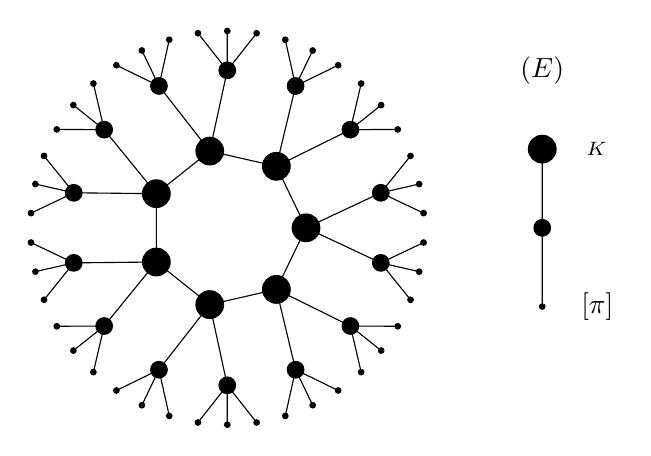
\begin{tikzpicture}
    \def\crater{7}
    \foreach \i in {1,...,\crater} {
        \draw[fill] (360/\crater*\i:1cm) circle (5pt);
        \draw (360/\crater*\i : 1cm) -- (360/\crater*\i+360/\crater : 1cm);
        \foreach \j in {-1,1} {
            \draw[fill] (360/\crater*\i : 1cm) -- (360/\crater*\i + \j*360/\crater/4 : 2cm) circle (3pt);
            \foreach \k in {-1,0,1} {
                \draw[fill] (360/\crater*\i + \j*360/\crater/4 : 2cm) --
                (360/\crater*\i + + \j*360/\crater/4 + \k*360/\crater/6 : 2.5cm) circle (1pt);
            }
        }
    }
    \begin{scope}[xshift=4cm]
    \node at (0,2) {$\End(E)$};
    \draw[fill] (0,1) circle(5pt) node[xshift=0.7cm]{$\Oc_K$} -- 
    (0,0) circle(3pt) --
    (0,-1) circle(1pt) node[xshift=0.7cm]{$\Z[\pi]$};
    \end{scope}
    \end{tikzpicture}
    \caption{An isogeny volcano with $\ell=3$; picture by De Feo}
    \label{picture_volcano}
\end{figure}

The case when $\left( \frac{\Delta_K}{p} \right)=1$ is the most interesting one to us; we can see that in this case the curves at the surface form a cycle, which is called the \emph{crater} of the volcano. We also give the following definition.
\begin{definition}
    Let $E/\F_q$ be an elliptic curve with trace of Frobenius $t$, and define $\Delta_K=t^2-4q$. We say that a prime $\ell\neq p$ is of Elkies type if $\left( \frac{\Delta_K}{\ell} \right)=1$.
\end{definition}

An example of an isogeny volcano with a crater can be seen in Figure \ref{picture_volcano}.

\subsection{The CM action}
We now recall an important feature of endomorphism rings of elliptic curves.

Let $\Oc$ be an order in an imaginary quadratic number field $K$, and denote by $Ell_q(\Oc)$ the set of $\F_q$-isomorphism classes of elliptic curves with \emph{complex multiplication} by $\Oc$, i.e. with $\End_{\F_q}(E)=\Oc$.

Given any curve $E\in Ell_q(\Oc)$ and an invertible ideal $\mathfrak{a}\subset\Oc$ with norm coprime to $q$, we can define the \emph{$\mathfrak{a}$-torsion} subgroup of $E$ as $$E[\mathfrak{a}]=\{ P\in E(\bar\F_q) \st \alpha(P)=0\;\forall\alpha\in\mathfrak{a} \}.$$

From this subgroup we can define a separable isogeny $\phi_{\mathfrak{a}}: E\to E/E[\mathfrak{a}]$. It turns out that this isogeny has degree equal to the norm of $\mathfrak{a}$, and its codomain is also an element of $Ell_q(\Oc)$; by composing with some purely inseparable isogeny we can define $\phi_{\mathfrak{a}}$ for any ideal.

Since the isogeny corresponding to the ideal $(f)$ is $f$ itself, we get an action of the class group $Cl(\Oc)$ (i.e. invertible ideals of $\Oc$ modulo principal ideals) on the set $Ell_q(\Oc)$, which we will denote by $\mathfrak{a}\star E$. We state the properties of this action in the following theorem.

\begin{theorem}
    Let $\F_q$ be a finite field and $\Oc\subset\Q(\sqrt{-D})$ an order in a quadratic imaginary field. Assume $Ell_q(\Oc)$ is non empty; then the action given by
    \begin{align*}
    Cl(\Oc)\times Ell_q(\Oc) & \to  Ell_q(\Oc)\\
    (\mathfrak{a}, E) & \mapsto  E/E[\mathfrak{a}]
    \end{align*}
    is free and transitive.
\end{theorem}

Coming back to volcanoes, we notice that this action gives us some information about the crater.

Assume that we have an elliptic curve $E/\F_q$ with Frobenius endomorphism $\pi$ and trace $t$, with $\End_{\F_q}(E)=\Oc_K$. Consider an Elkies prime $\ell$; then the characteristic polynomial splits modulo $\ell$ as $\pi^2-t\pi+q\equiv(\pi-\lambda)(\pi-\mu)\pmod\ell$ for two distinct eigenvalues $\lambda,\mu$.

If we associate to $\lambda,\mu$ the ideals $\mathfrak{a}=(\ell,\pi-\lambda)$ and $\bar{\mathfrak{a}}=(\ell,\pi-\mu)$ inside $\Oc_K$, we see that $E[\mathfrak{a}]$ is precisely the eigenspace relative to $\lambda$ for the action of Frobenius on $E[\ell]$, and $E[\bar{\mathfrak{a}}]$ is the eigenspace of $\mu$.

Since $\mathfrak{a}\bar{\mathfrak{a}}=\ell\Oc_K$, the two ideals are inverses in $Cl(\Oc_K)$, meaning that the isogenies $\phi_{\mathfrak{a}}:E\to \mathfrak{a}\star E$ and $\phi_{\bar{\mathfrak{a}}}:\mathfrak{a}\star E\to E$ are dual; thus the two eigenvalues $\lambda,\mu$ define two opposite directions of walking around the crater of the isogeny volcano to which $E$ belongs.

Coming back to supersingular curves, we will see some theorems that will help us translate the volcanoes setting to the supersingular case. First of all, recalling theorem \ref{thm_endfp}, we have that:

\begin{proposition}
    Let $E/\F_p$ be a supersingular elliptic curve and $\End_{\F_p}(E)$ denote the ring of $\F_p$-rational endomorphism of $E$. Then $$\Z[\pi]\subset \End_{\F_p}(E) \subset \Q(\sqrt{-p}).$$
\end{proposition}

We recall that in the case $p\equiv1\pmod 4$ the maximal order of $\Q(\sqrt{-p})$ is $\Z[\sqrt{-p}]$, while if $p\equiv 3\pmod 4$, the maximal order is $\Z[\frac{\sqrt{-p}+1}{2}]$. This means that in the first case $\End_{\F_p}(E)$ must be $\Z[\pi]$, while in the second case it can be either $\Z[\pi]$ or $\Z[\frac{\pi+1}{2}]$.

Finally, we can use the terms horizontal, ascending and descending for an isogeny $\phi:E\to E'$ as for ordinary curves, respectively if $\Oc=\Oc'$, $\Oc\subset\Oc'$ or $\Oc\supset\Oc'$.

We then have the following result, which basically states that $Ell_p(\Oc)$ is a cycle. 

\begin{theorem}[\cite{Delfs_Galbraith}]\label{CSIDH_cycle}
    Let $p\ge 5$ be a prime with $p\equiv3\pmod{4}$, and let $2<\ell\neq p$ another prime. Then the supersingular component of $G_\ell(\F_p)$ has two levels, and if $\ell$ is an Elkies prime each vertex has two horizontal $\ell$-isogenies.
\end{theorem}



\section{Montgomery models}
\cite{Costello_Montgomery} from \cite{Montgomery_curve}.

